\documentclass[12pt]{article}
\usepackage{multicol}
\usepackage{apacite}
\usepackage{graphicx}
\usepackage{setspace}
\usepackage{amsmath}
\usepackage{mathtools}
\usepackage{fixltx2e}
\usepackage{listings}
%\usepackage{appendix}
\lstdefinelanguage{JavaScript}{
  keywords={typeof, new, true, false, catch, function, return, null, catch, switch, var, if, in, while, do, else, case, break},
  keywordstyle=\color{blue}\bfseries,
  ndkeywords={class, export, boolean, throw, implements, import, this},
  ndkeywordstyle=\color{darkgray}\bfseries,
  identifierstyle=\color{black},
  sensitive=false,	
  comment=[l]{//},
  morecomment=[s]{/*}{*/},
  commentstyle=\ttfamily,
  stringstyle=\ttfamily,
  morestring=[b]',
  morestring=[b]"
}
\lstset{
  language=JavaScript,
  aboveskip=3mm,
  belowskip=3mm,
  showstringspaces=false,
  columns=flexible,
  basicstyle={\small\ttfamily},
  numbers=none,
  breaklines=true,
  breakatwhitespace=true
  tabsize=4
}
\DeclareGraphicsExtensions{.pdf,.svg,.png,.jpg}

% start the document
\begin{document}

% title page for thesis
%\title{Visualizing and Refining Connectivity Map Query Results}
%\maketitle
%\begin{titlepage}
%\begin{center}
%Proposal for a\\
%Thesis in the Field of\\
%Biotechnology\\[\baselineskip]
%In Partial Fulfillment of the Requirements\\
%for a Master of Liberal Arts Degree\\[\baselineskip]
%Harvard University\\
%Extension School\\[\baselineskip]
%Theodore Natoli\\
%51 Lewis Avenue, Apartment 3\\
%Arlington, MA 02472\\
%857-498-1946\\
%\texttt{tnatoli@fas.harvard.edu}\\[\baselineskip]
%Proposed Start Date: \today\\
%Anticipated Date of Graduation: \today\\
%Thesis Director: Aravind Subramanian
%\end{center}
%\end{titlepage}
% end of title stuff

% title page for proposal
\begin{titlepage}
\begin{center}
A Method for Connectivity Map\\
Query Result Refinement and Visualization\\[\baselineskip]
Theodore E. Natoli\\[\baselineskip]
A Thesis in the Field of Biotechnology\\
for the Degree of Master of Liberal Arts in Extension Studies\\[\baselineskip]
Harvard University\\[\baselineskip]
September 2014\\[\baselineskip]
\end{center}
% blank page here
\newpage
\mbox{}
\end{titlepage}

%\section{Tentative Title}
%\title{Tentative Title: Visualizing and Refining Connectivity Map Query Results}
%\maketitle

% begin double spacing
\doublespacing

\section{Abstract}
The Connectivity Map (CMap) is a database of gene expression signatures obtained from experiments in which cultured human cells are treated with pharmacologic and genomic perturbagens. A typical use case of this database is for a researcher to query with a signature of a cell state of interest and use the matching perturbagens to develop a functional hypothesis for follow-up. Current pattern matching algorithms that perform CMap queries suffer from a universal weakness -- the enormous size and richness of signatures in CMap means that a query typically generates hundreds of strong connections. These connections are hard to distinguish, thereby making prioritization difficult. An interconnectivity-based method of query result refinement, whereby query results that are highly interconnected amongst themselves are highlighted over singletons, proves an effective solution to the prioritization problem. To implement this method, I built a web-based tool that displays CMap query results visually in a graph layout and helps identify highly interconnected sub-groups of signatures. Using this tool and a set of curated queries, I have verified that highly interconnected query results are frequently biologically relevant and occur much more frequently than would be expected by chance alone. The tool has also proved useful in enabling hypothesis generation for novel queries.

% blank page here
\newpage
\mbox{}

% table of contents here
\tableofcontents

% list of tables
%\listoftables

% list of figures
\listoffigures

\section{Introduction}

\subsection{The Research Problem}

The CMap database, built and maintained at The Broad Institute, is a compendium of gene expression signatures resulting from the treatment of cultured human cells with perturbations such as small molecule compounds (CP), short hairpin RNAs (shRNA), or over-expression constructs (OE). The utility of the CMap database is that of a gene expression search engine. Users are able to pose questions about relationships between cellular states and formulate hypotheses based on similarities or differences in the states' gene expression signatures, or the sets of genes that are differentially regulated by a particular perturbation.

Hypotheses are generated by posing search queries into the database and examining the query results. A CMap query is a focused question in which a user inputs a gene expression signature, called the query, and computes the similarity, or connectivity, between his/her query and other signatures in the database. Positive connectivity indicates that two signatures' expression changes are similar and vice versa. Researchers can use CMap to find connections between signatures within or external to the database. Hypotheses may be in the form of ``the shRNA knockdown of gene X connects to shRNA knockdown signatures of pathway Y members, so X is probably a member of Y.'' Or perhaps ``the signature of compound Z connects to the knockdown signature of gene X, so perhaps X is the target of Z.''

Lamb et al. demonstrated a more directly therapeutically relevant use of the original incarnation of CMap when they discovered that the signature of sirolimus connected strongly to a signature of dexamethasone sensitivity. Dexamethasone is a treatment for acute lymphoblastic leukemia (ALL), but many patients eventually become resistant to it\cite{tissing_molecular_2003}. The CMap connection between sirolimus and dexamathasone sensitivity suggested that sirolimus might be effective in reversing resistance in ALL patients who had become resistant to dexamethasone. A follow-up experiment confirmed that sirolimus conferred dexamathasone sensitivity to CEM-c1 cells, a previously dexamethasone-resistant cell line \cite{lamb_connectivity_2006}. 

The CMap database contains over 400,000 signatures spanning over 70 cell types. Because of this large size, interpreting and prioritizing query results has become difficult. For example, accepting only the top one percent of connections yields nearly 4,000 signatures. Follow-up on such a large number of primary hits is nearly impossible in most cases. However, within a set of initial query results, there frequently exists a set or sets of signatures that are more tightly interconnected with themselves than with other signatures. These interconnected sets are more likely to be indicative of robust biological signal and should therefore be prioritized over other singleton connections. The goal of this work was to build a web-based tool to implement an algorithm to identify subsets of high interconnectivity within lists of initial query results and to visualize the relationships between these subsets in a graph layout. This tool is useful in refining initial CMap query results into smaller, more actionable lists of connections that can be further investigated in secondary assays.

% key terms
%\section{Definition of Terms}
%\begin{enumerate}
%\item Gene expression profiling: the parallelized collection of many simultaneous gene expression measurements.
%\item Gene set enrichment analysis (GSEA): an approach used to test for a gene set's overall trend towards the extremes of a ranked-list of genes.
%\item Kolmogorov-Smirnov (KS) statistic: a statistical measure used to quantify the trending of one group's members towards the extremes of another group's distribution.
%\item Graphical model: a computational tool for approximating the interrelationships between a set of objects.
%\item Connectivity Map (CMap): a database of gene expression signatures spanning many treatment types and cell contexts.
%\item CMap connection: a quantified similar or dissimilar relationship between two gene expression signatures.
%\end{enumerate}


\subsection{Gene Expression Profiling}

Gene expression profiling is the simultaneous measure of the RNA transcript levels of many genes within a cell or group of cells. These measurements can help to provide insight into the cellular state or states of the cells in question. For example, if many cell-cycle genes are observed to be active, it could suggest that the cells are actively dividing. Conversely, if many apoptotic genes are active, the cells might be dying. Frequently, the goal of gene expression profiling is to identify genes that are differentially regulated between one or more sets of conditions. For example, one might measure expression in cells that have and have not been treated with a drug of interest, and then compare the resulting expression profiles to identify genes that are substantially up- or down-regulated in the treated cells relative to the untreated. Current technologies, such as the microarray, allow for many such gene expression experiments to be run in parallel, enabling the comparative analysis of hundreds or thousands of expression profiles corresponding to an equal number of experimental conditions. Similarly, expression profiling can be used to identify genes differentially regulated between disease and normal states. van't Veer et al. used gene expression profiling to identify a set of genes that were predictive of breast cancer metastasis \cite{van_t_veer_gene_2002}. Because of its ability to identify such signatures, gene expression profiling is a powerful and often-used tool in contemporary biology.

\subsection{Gene Set Enrichment Analysis (GSEA)}

Gene Set Enrichment Analysis (GSEA) is an analytical approach designed to extract biological insight from gene expression data \cite{subramanian_gene_2005}. It leverages  groups of genes, called gene sets, that share some biological commonality (i.e. members of a cellular signaling pathway) and computes their enrichment, or trend towards the top or bottom, of a ranked list of genes generated by comparing expression profiles across two experimental classes (i.e. tumor vs. normal). For example, one might define many sets of genes, each corresponding to a cellular pathway. One could then rank-order all genes by their differential expression when comparing profiles of tumor vs. normal samples. Lastly, one could compute the enrichment of each pathway in the rank-ordered list to attempt to identify pathways that might be active in the particular tumor in question.

Mechanically, GSEA computes a Kolmogorov-Smirnov (KS)\\
 statistic when comparing a given gene set to a given ranked list \cite{hollander_wolfe_1975}. Effectively, this amounts to walking down the ranked list, increasing a running-sum statistic when one encounters a gene in the gene set and decreasing it for genes not in the gene set. The magnitude of the increment depends on the correlation of the gene with the phenotype. The enrichment score is the maximum deviation from zero encountered in the walk \cite{subramanian_gene_2005}. GSEA has been used extensively for identifying coherent sets of genes that are collectively modulated under certain disease states and/or experimental conditions. In fact, a GSEA software suite and an accompanying online database exist to facilitate comparisons between novel and curated gene sets \cite{msigdb_website}.

\subsection{The Connectivity Map}

The Connectivity Map (CMap) is a database containing the gene expression signatures resulting from treating cultured cells with various chemical and genomic perturbations \cite{lamb_connectivity_2006}. The purpose of CMap is to serve as a lookup table of functional annotation. These annotations might be derived by comparing signatures within the CMap database or by querying the database with externally generated signatures. The database itself can be thought of as a large matrix where each row is a gene and each column is an experiment in which a particular perturbagen was profiled under a given set of conditions (i.e. cell context, dose, treatment time, etc.). The values in the matrix are differential expression measures generated by comparing the expression levels of the genes across perturbed and control states. Thus, each column of the matrix can be thought of as a given perturbagen's expression signature.

\subsubsection{Computing Connections in the Connectivity Map}

A primary use of the CMap database is to compare the signatures of different perturbations and to assess their similarity. Perturbagens that, when used to treat cultured cells, result in similar gene expression consequences will yield similar CMap signatures. Such signatures are said to be positively connected in the CMap sense. Conversely, perturbagens that elicit inversely related expression consequences are said to be negatively connected. For a given query signature Q and a reference signature R, the weighted connectivity score (WTCS) is computed by computing and integrating two KS statistics, one each for the n most up- and down-regulated genes in Q. The algorithm proceeds as follows:
\begin{enumerate}
\item Order Q
\item compute ES\textsubscript{up} as the enrichment of the n most up-regulated genes in R
\item compute ES\textsubscript{dn} as the enrichment of the n most down-regulated genes in R
\item compute WTCS as 
\begin{enumerate}
	\item 0 if ES\textsubscript{up} and ES\textsubscript{dn} share the same sign
	\item $ \frac{|ES\textsubscript{up}| + |ES\textsubscript{dn}|}{2} $, where the resulting WTCS is given the sign of ES\textsubscript{up} if ES\textsubscript{up} and ES\textsubscript{up} are of different signs.
\end{enumerate}
\end{enumerate}

WTCS will be positive for signatures that are positively related and negative for those that are inversely related.

A common CMap use case is to select a given query signature Q from the database and compute its similarity to all other signatures. The remaining signatures can be ranked according to their connection strength with Q. The connections can be used to gain insight and form hypotheses about Q. For example, if Q is a signature of a novel compound and it connects strongly to signatures of compounds of a known pharmacological class, one might hypothesize that the novel compound is also a member of this class. Similarly, if Q connects strongly to the knockdown signature of gene G, one might hypothesize that G is the novel compound's target. Q need not be a signature from the CMap database. For instance, it might be the signature of some disease and one might seek connections to genes whose modulation could be causing the disease or to compounds that could have therapeutic relevance. 

\subsection{Graphical Depictions of Biological Phenomena}

In the fields of computer science and mathematics, a graph is a means by which to represent a set of objects and the relationships between them. It is frequently depicted as a set of nodes, where each node represents an object. Connections, where they exist, are represented by edges (Figure ~\ref{fig:graph}).


% example graph image
\begin{figure}[h]
\centering
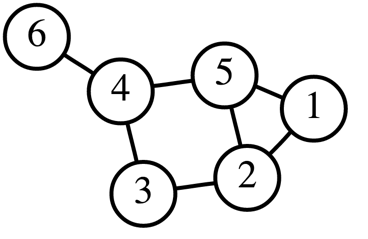
\includegraphics[scale=0.5]{img/graph_example.png}
\caption{An example of a graph. The six nodes are connected by seven edges. All nodes other than node 6 have at least two edges. An edge between two nodes indicates an interaction or relationship between the nodes.}
\label{fig:graph}
\end{figure} 

Although they originated in other fields, graphs have frequently been used as tools to model biological phenomena. Graphical models of protein interaction networks, gene expression networks, and other similar phenomena are commonplace. Friedman used graphical models to infer and visualize gene regulatory networks \cite{friedman_inferring_2004}. Lage et al. used graphical models to characterize existing and elucidate novel protein-protein interaction networks \cite{lage_human_2007}. Because of its widespread use and adoption, the graphical model is an appropriate, familiar, and effective means to depict connectivity between CMap perturbagens.
In the graph visualization generated by QViz, CMap perturbagens are represented as nodes. Where a connection exists between to perturbagens, a line is drawn connecting their nodes. Thus, the user is able to easily see which perturbagens are connected to each other and can easily identify highly interconnected subsets of perturbagens, if they exist. 
 
% high-level view of the app
%\section{The QViz Application}



% methods
\section{Methods}
\subsection{Computing and Visualizing Connections}

In order to improve the performance of the web application, all connections between CMap signatures were pre-computed using WTCS and stored in a database so the application can simply look them up without any computation. These connections were then summarized using the summly algorithm, which scores connections based on their consistency across multiple cell contexts \cite{subramanian_summly}. The WTCS scores are converted to a rank point scale, or a normalized percentile rank, rescaled to range between -100 and 100, where 100 is completely positively connected and 100 is completely negatively connected. Connections that are maintained across many cell types receive a higher magnitude rankpoint than those that occur in only a small number. An additional benefit of applying the summly algorithm is that it abstracts away the concept of cell type and provides a more perturbagen-centric view of connectivity, thus dramatically reducing the connectivity space. The CMap database contains over 450,000 signatures, but that is reduced to a little over 7,000 perturbagens when considering only those that produced repeatable signatures in enough cell lines, in this case 4, to be considered for summly. The summly scores were precomputed and are stored in a database that the application uses to simply look up connectivity scores instead of computing them on-the-fly. 
Users interact with the application by inputting a list of perturbagens that have resulted from running a CMap query. QViz then searches the database for the summly scores that exist between all pairwise combinations of these perturbagens. QViz displays the perturbagens as nodes in a graph. Where the summly score between two nodes exceeds a given threshold, the application asserts that a connection exists between the perturbagens, and a line is drawn between them. Users are able to tune the summly score threshold to achieve the desired level of stringency in connection calling. In addition to displaying the graph, QViz also computes the clique density of the graph, and the size and members of the largest clique. It supplies p-values for each of these metrics. Please see the section below for how the p-values are computed. A clique, or fully connected subgraph, is a subset of a graph whose members all share a connection to each other \cite{luce_method_1949}. The clique density is computed is the number of cliques divided by the total number of nodes, and it can be thought of as a proxy for the interconnectedness of a graph. For example, if graphs A and B have the same number of nodes but graph A has twice as many cliques as graph B, then graph A has twice the clique density and is therefore twice as interconnected. Additionally, because the clique density metric is normalized to account for the number of nodes in a graph, it can be used to compare the interconnectedness across graphs of different sizes. 

\subsection{Estimating Significance}
QViz computes the clique density and the size of the largest clique for each set of perturbagens input by the user, but these metrics are difficult to interpret without an accompanying measure of significance. For example, a clique density of 1.5 is somewhat meaningless without a sense of how frequently a value of 1.5 or higher is achieved in general. To assess the frequency of clique density value occurrences, it is necessary to build a reference distribution of clique density values. This reference distribution was constructed by computing the clique densities of the connections resulting from querying the CMap database with 1,000 randomly selected signatures of dimethylsulfoxide (DMSO) treatment. DMSO is a solvent that is frequently used to dissolve and deliver compound treatments to cultured cells. Hence, the signature of treating with DMSO alone serves a relevant negative control for many perturbagen signatures. 
Figure XX below shows the distribution of clique density values for DMSO query results across a small range of graph sizes and rank point thresholds. Such a distribution was computed for graph sizes between 2 and 100 and rank point thresholds from 90 to 99. Each QViz analysis will result in a clique density D based on the number and identity of the user's list of input perturbagens and the rank point threshold they have selected. The application computes the p-value, or the probability of observing a clique density at least as extreme as V by computing the proportion of of clique density values more extreme than V from the DMSO distribution at the same perturbagen number and rank point threshold. For example, a density of D and a p-value of 0.05 indicates that in the DMSO distribution, 5\% of the observed values were greater than equal to D. In the same fashion, the DMSO distributions are used to compute p-values for the largest clique size. 


\subsection{Other Application Features}
At a high level, QViz allows users to input their CMap query results, visualize them as a graph, and identify subsets that may be highly interconnected. In order to maintain reasonable performance, the application allows the user to input a maximum of 100 perturbagens. Once the graph is computed and drawn, QViz highlights and lists the members of the largest clique in the graph so that the user is able to easily identify them. The user is able to hover over each graph node to see the name of the corresponding perturbagen. He or she can also change the cursor to a selection brush and can drag the mouse to highlight multiple nodes and see the names of their corresponding perturbagens. QViz provides a search box so that the user can input the names(s) of perturbagens to search for and highlight within the graph. The nodes of the graph can be dragged and repositioned so that the user can isolate particular nodes. 
QViz has a `take a tour' feature that walks the user through each of the application's components. It also has a list of pre-selected, curated sets of perturbagens, or example sets, that users can select to see an example use of the application. These example sets include the top XX connections resulting from CMap queries with expression signatures of the following compounds:

\begin{enumerate}
\item MEK inhibitior
\item PI3K/MTOR inhibitior
\item HMGCR inhibitior
\item Glucocorticoid agoniist
\item Proteasome inhibitor
\end{enumerate}

These example sets were selected such that each contains at least a single well-connected subgroup. Hence, they help give the user a feel for the level interconnectedness achievable for highly biologically relevant queries.

% app screen shot image
%\begin{figure}[h]
%\centering
%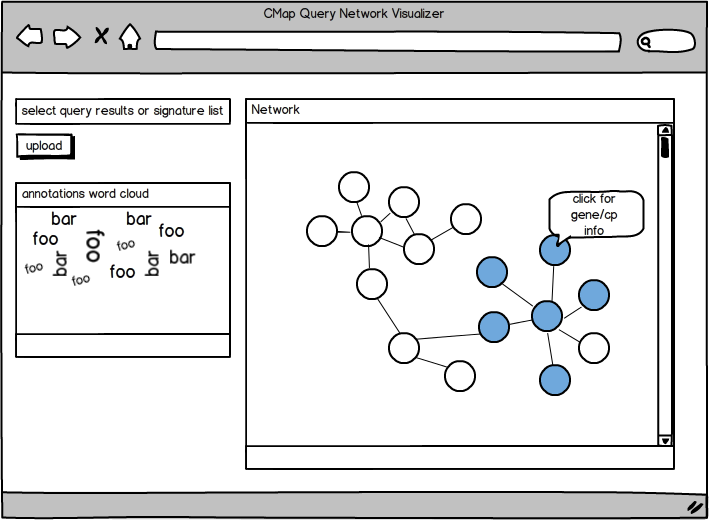
\includegraphics[scale=0.5]{img/app_mockup.png}
%\caption{Application mockup. The application will have a main viewing area in which the graph will be displayed. The user will be able to see various signature clusters highlighted and generate a word cloud visualization from metadata of selected signatures in a smaller viewing area. Hovering the mouse over a node will display metadata about the corresponding signature. There will also be a small input box for the user to upload lists of query results.}
%\label{fig:app_mockup}
%\end{figure}


\subsection{Software Components}
\subsubsection{Front End: HTML \& D3.js}

Hypertext markup language (HTML) is and has been the standard language for displaying information over the Internet within web browsers. HTML5, the most recent revision of the HTML standard, is used as the framework QViz. HTML5 offers many useful features for application development and is supported by most modern web browsers \cite{w3c_html5}. 

To support user interaction, the graph visualization is built using D3.js, a JavaScript library for data visualization. Created by Mozilla in 1995, JavaScript is a programming language that is interpreted by most modern web browsers and allows developers to create interactive elements within web pages \cite{mozilla_javascript}. D3, short for Data Driven Documents, is a JavaScript library written by Mike Bostock and designed specifically to enable rich and interactive data visualizations \cite{bostock_d3}. D3 is particularly well-suited for visualizing CMap connections because of its ability to easily integrate and bind data to on-screen elements. It has been used in many similar projects and is capable of generating the graph of visualizations in QViz.

% d3 graph image
%\begin{figure}[h]
%\centering
%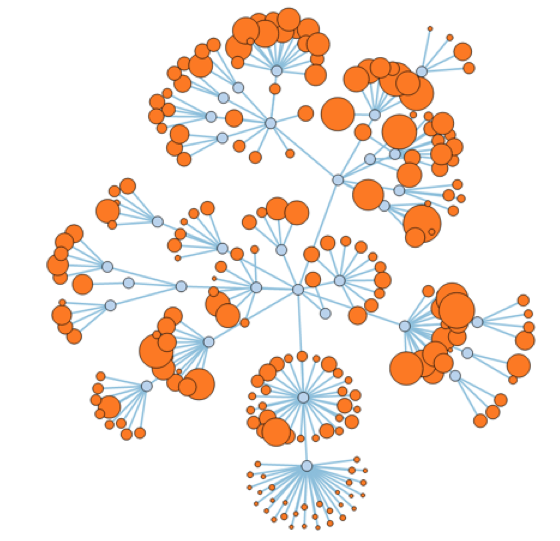
\includegraphics[scale=0.5]{img/d3_graph_example.png}
%\caption{A graph generated using D3.js}
%\label{fig:d3_graph_example}
%\end{figure}

% d3 word cloud image
%\begin{figure}[h]
%\centering
%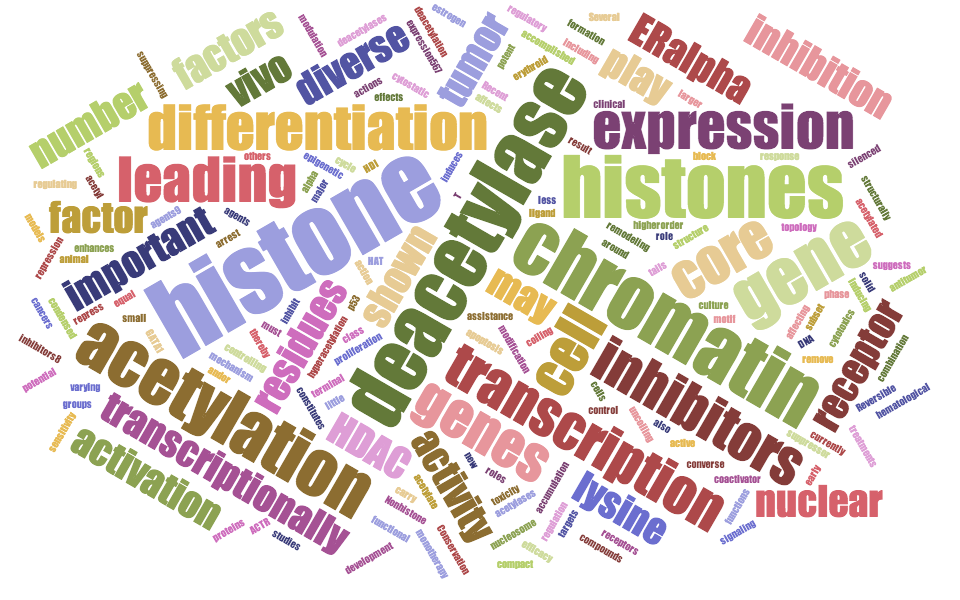
\includegraphics[scale=0.5]{img/d3_word_cloud_example.png}
%\caption{A word cloud generated using D3.js. The size and color of the words can be used to encode information, such as frequency of occurrence or position relative to other parts of speech.}
%\label{fig:d3_word_cloud_example}
%\end{figure}

\subsubsection{Back End: MongoDB, R, and Node.js}

MongoDB is a database system developed by MongoDB Inc. Unlike traditional Structured Query Language (SQL) database systems that require rigid data storage schema, MongoDB's schema is very loose and fluid. Rather than storing data in tables that may or may not be linked to each other, MongoDB stores data in ``collections,'' where each collection is simply a list of ``documents.'' Documents are simply data objects that can have any number of attributes and each document need not have the same attributes as others \cite{mongodb}. Perhaps the main benefit of using MongoDB is that it natively stores data in JavaScript Object Notation (JSON) format \cite{json}. JSON is the data object format used by JavaScript, so using MongoDB to store the connectivity data means that when the application queries MongoDB, the database will respond with data in a format the application can easily handle.

% describe mongo schema
MongoDB documents are simply JSON objects. These objects contain key-value pairs and the values can be accessed by providing the appropriate keys, or attributes. A CMap connection can be modeled as a very simple JSON object with the following attributes:

\begin{enumerate}
\item perturbagen 1
\item perturbagen 2
\item rankpoint
\end{enumerate}

An example CMap connection stored as a JSON document might look like this:

\begin{lstlisting}
{
	"perturbation_1": "vorinostat",
	"perturbation_2": "trichostatin-a",
	"rankpoint": 98.0
}
\end{lstlisting}
	
In the example above, vorinostat and trichostatin-a have a connection strength of 98.0. Providing the names of the two perturbagens is enough to uniquely identify this and any CMap summly connection. MongoDB allows for searching over the values of all documents that contain a given key or set of keys. QViz stores each CMap connection as a document in a single MongoDB collection. Based on the user's input set of query results (perturbagen names), MongoDB is able to retrieve all connections between the query results by looking up all documents where the perturbagen\_1 and perturbagen\_2 fields are members of the input query result set and then return the results to the application as a JSON object.

R is a programming language for statistical analysis. It was developed in 1997 by Ross Ihaka and Robert Gentleman and has since become widely used in many analytical computing applications \cite{r_lang}. It has a large community of developers who contribute packages and utilities to perform specific analyses. In this work, the `igraph' package is used to compute the clique properties of the graphs generated by QViz. This package is appealing for the QViz use case because it contains built-in functions that compute the number of cliques and the size and number of the largest cliques in a graph, among other useful features \cite{igraph}.

Node.js is a JavaScript-based platform for web server development. It implements an event-driven paradigm, which means that it enables writing programs built for quickly responding to inputs from a user or another application \cite{node}. In this project, Node.js acts as the web server that handles requests from the web application and query responses from MongoDB. It acts as the middle layer that shuffles data between MongoDB, where it is stored, R, where it is analyzed, and the web application, where it is displayed. Figure ~\ref{fig:app_data_flow} illustrates how data flows through the various front and back end layers of the application. Node.js is appealing for this use case because, like MongoDB and D3, it is based in JavaScript. It therefore allows for easily passing query parameters from the application to MongoDB and query results as JSON objects from MongoDB to the application.


% figure showing app data flow
\begin{figure}[h]
\centering
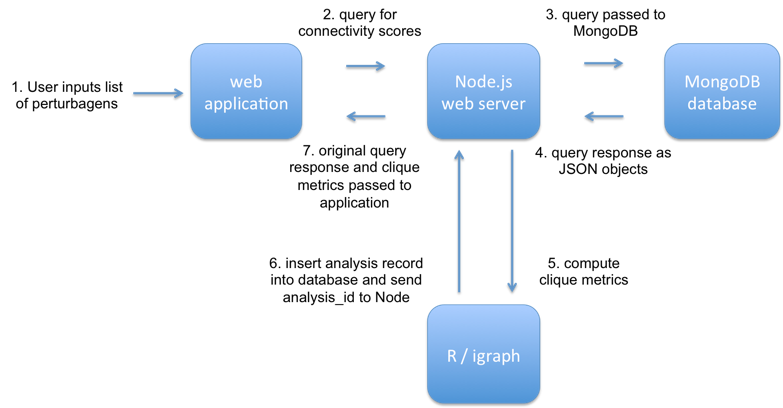
\includegraphics[scale=0.5]{img/app_data_flow_small.png}
\caption{ NEEDS TO BE UPDATED: Application data flow diagram. The application receives a list of perturbagens from the user. It then sends a query for these perturbagens' connectivity scores to Node.js. Node.js receives the query, passes it to MongoDB, and waits for the response. Once the JSON response is received, Node.js passes it back to the application for visualization.}
\label{fig:app_data_flow}
\end{figure}


% results
\section{Results}

\subsection{Highly Interconnected Query Results are Frequently Biologically Relevant}
Lorem ipsum dolor sit amet, consectetur adipisicing elit, sed do eiusmod tempor incididunt ut labore et dolore magna aliqua. Ut enim ad minim veniam, quis nostrud exercitation ullamco laboris nisi ut aliquip ex ea commodo consequat. Duis aute irure dolor in reprehenderit in voluptate velit esse cillum dolore eu fugiat nulla pariatur. Excepteur sint occaecat cupidatat non proident, sunt in culpa qui officia deserunt mollit anim id est laborum.

\subsection{Application Efficiently Identifies Interconnected Results}
Lorem ipsum dolor sit amet, consectetur adipisicing elit, sed do eiusmod tempor incididunt ut labore et dolore magna aliqua. Ut enim ad minim veniam, quis nostrud exercitation ullamco laboris nisi ut aliquip ex ea commodo consequat. Duis aute irure dolor in reprehenderit in voluptate velit esse cillum dolore eu fugiat nulla pariatur. Excepteur sint occaecat cupidatat non proident, sunt in culpa qui officia deserunt mollit anim id est laborum.

\subsection{Novel Query Results That Show Interconnectivity}
could be useful to talk about ERG here

Lorem ipsum dolor sit amet, consectetur adipisicing elit, sed do eiusmod tempor incididunt ut labore et dolore magna aliqua. Ut enim ad minim veniam, quis nostrud exercitation ullamco laboris nisi ut aliquip ex ea commodo consequat. Duis aute irure dolor in reprehenderit in voluptate velit esse cillum dolore eu fugiat nulla pariatur. Excepteur sint occaecat cupidatat non proident, sunt in culpa qui officia deserunt mollit anim id est laborum.



% summary and conclusions
\section{Summary and Conclusions}
Lorem ipsum dolor sit amet, consectetur adipisicing elit, sed do eiusmod tempor incididunt ut labore et dolore magna aliqua. Ut enim ad minim veniam, quis nostrud exercitation ullamco laboris nisi ut aliquip ex ea commodo consequat. Duis aute irure dolor in reprehenderit in voluptate velit esse cillum dolore eu fugiat nulla pariatur. Excepteur sint occaecat cupidatat non proident, sunt in culpa qui officia deserunt mollit anim id est laborum.

challenges, things that could still be improved

also possible to input an arbitrary list. maybe mention this in discussion

app is built on summly space, but possible to use any arbitrary space. could be a potential extension 



% challenges
%\section{Research Limitations}
%\subsection{Storing Entire Connectivity Matrix in MongoDB}

%The CMap database contains over 400,000 signatures. Thus, the matrix of all pairwise connectivity values would be 400,000 x 400,000, or 160 billion unique values. Such a matrix would translate to a MongoDB collection of 160 billion documents. A collection of that size may prove time-consuming to query and could result in substantial lag times experienced by the application end-user. There are several options for mitigating this issue, should it arise. The first is to use only a subset of the matrix. CMap provides a high- or low-quality label to each of their signatures. There are roughly 240,000 high-quality signatures, so using only those would reduce the size of the MongoDB collection to 62.5 billion. Another alternative is to use an abstracted view of the signatures. The CMap group is developing a summarized set of perturbation-centric signatures where connections between perturbations are collapsed across cell lines. The current summarized space is approximately 8,000, which would yield a MongoDB collection of 64 million, a roughly thousand-fold reduction in database size. An advantageous byproduct of using the summarized space is that it would abstract away the notion of cell context and might make connectivity results easier to interpret for the end-user.

%\subsection{Displaying Large Graphs in a Web Browser}

%There may be an upper limit to the number of nodes that can be displayed within a modern web browser while still allowing for reasonable application performance. This number may vary depending on the capabilities of the end-user's computer, but testing across a few computers, each with different specifications, should yield a rough estimate of a reasonable graph size. It may be problematic if this size is well below the number of highly interconnected signatures within a given query result. If this were the case, the application would not be able to display all meaningful nodes simultaneously. Options for mitigating this issue include implementing a pan or zoom feature that would allow users to see only portions of the entire graph at a time or computationally collapsing nodes to reduce the overall number to a more manageable size. Both options could potentially increase application development time and computational burden on the end-user's machine and will need to be considered carefully if not all meaningful connections can be displayed simultaneously.

%\subsection{Incorporation of Signature Metadata}

%Each CMap signature is accompanied by a set of metadata that describe how the signature was generated. This information includes the perturbation profiled and other experimental parameters such as treatment time, dose, and cell line. It is this information that will be necessary for generating the word cloud visualization and other mouse-over interactions in the application. The CMap group has made this data available through an Application Programmer Interface (API), but accessing this means that my application will need to interact with a second database. Such a configuration is certainly possible, but could potentially increase lag time experienced by the end-user. If the lag time is prohibitive, it might be necessary to forego the metadata-based components of the visualization.


% timeline

% bibliography
\bibliographystyle{apacite}
\bibliography{Natoli_T_ALM_Biotech_Thesis}

\section{Appendix A: Source Code}

\subsection{CSS}

\subsection{HTML}

\subsection{JavaScript}

\subsection{R}





\end{document}